\section{Fazit}
\label{sec:schluss}

Der Bundesverband Musikindustrie e.V. prognostiziert für physische Tonträger
(CD, DVD, ...) einen Umsatzrückgang von 1,1 Mrd. \euro{} im Jahr 2013 auf 800
Mio. \euro{} im Jahr 2018 (\autoref{fig:umsatzprog}). Gleichzeitig gewinnen
Musikangebote über das Internet (Downloadportale und Streaming-Angebote) an
Bedeutung. Bis 2018 wird der Anteil der Internetangebote am Gesamtumsatz von
22,6\% in 2013 auf 50\% steigen und damit gleichauf mit dem Umsatzanteil von
physischen Datenträgern (49,4\%) liegen.

\begin{figure}[h]
    \begin{center}
        \begin{minipage}[t]{\textwidth}
            \begin{center}
                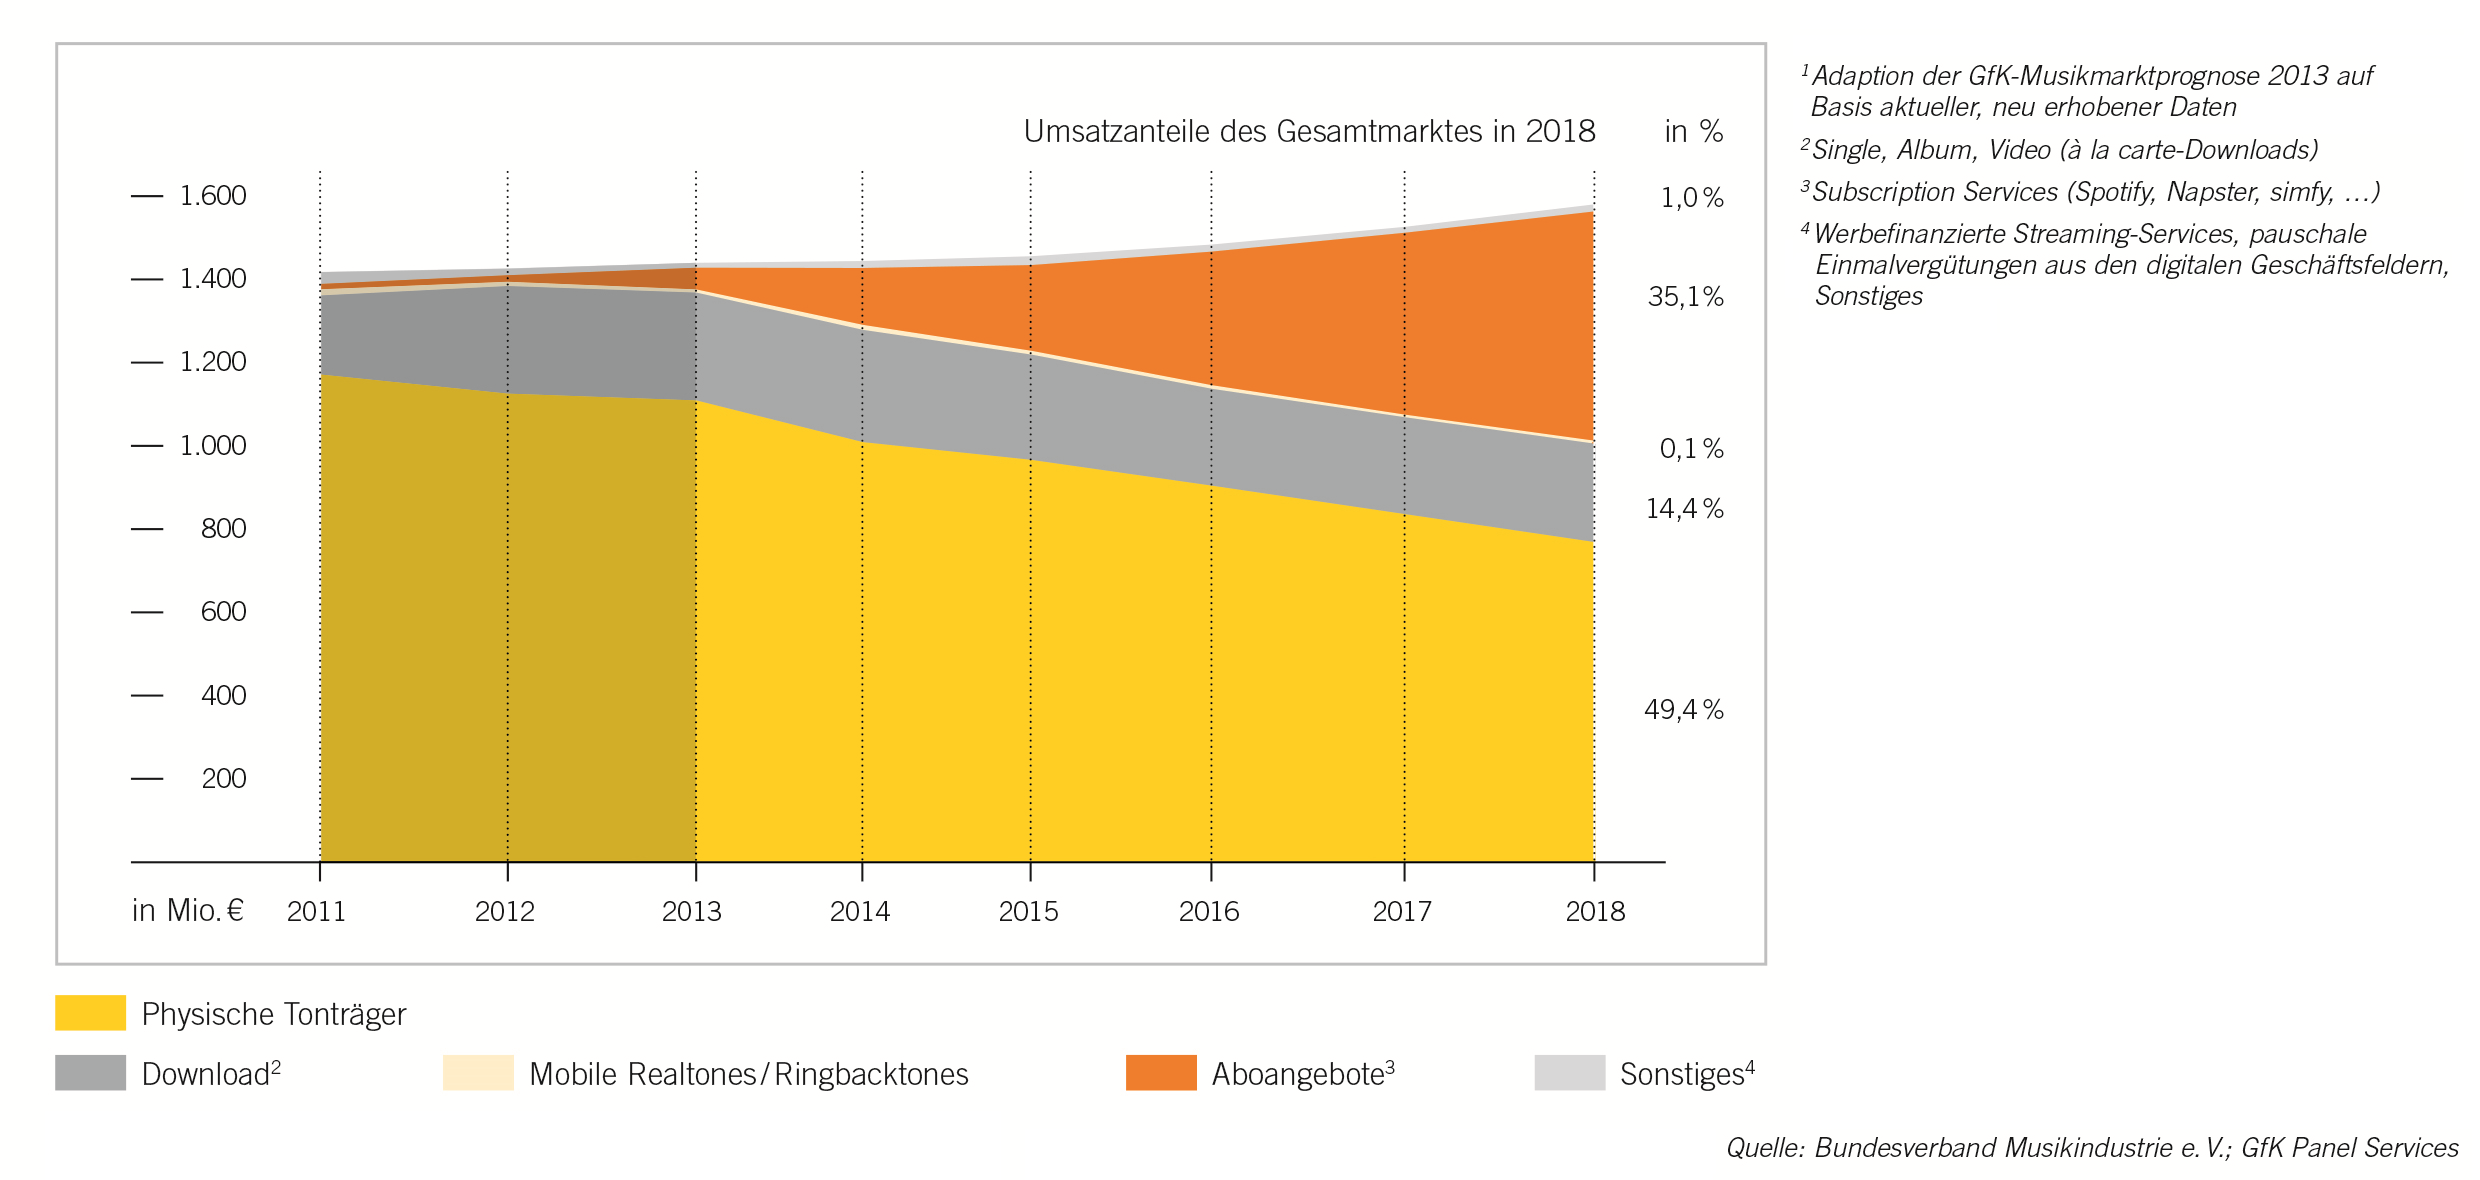
\includegraphics[width=\textwidth]{Bilder/Schluss/prognose.png}
                \caption[Prognose für die Umsatzanteile bis 2018 \newline \url{http://www.musikindustrie.de/uploads/media/140325\_BVMI\_2013\_Jahrbuch\_ePaper\_V02.pdf} S.15 (zuletzt aufgerufen am 03.08.2015)]{Prognose für die Umsatzanteile bis 2018}
                \label{fig:umsatzprog}
            \end{center}
        \end{minipage}
    \end{center}
\end{figure}

Internetangebote werden aber auch für die Film- und Fernsehindustrie immer
wichtiger: viele Sender betreiben Mediatheken mit den aktuellen
Fernsehsendungen; statt eine DVD oder Blue-Ray-Disc zu kaufen oder auszuleihen
werden Filme aus Videoportalen wie Maxdome und Amazon Prime geladen; Netflix
bietet Serien und Filme ausschließlich online an.

Um bei hochauflösenden Filmen lange Wartezeiten und \glqq Ruckler\grqq{} zu
vermeiden, sind hohe Übertragungsraten auch für Privathaushalte notwendig. Diese
Bandbreiten werden u.a. erreicht, indem Privathaushalte über Kabel aus polymer
optischer Fasern an Glasfasernetze angeschlossen werden.

Transparente Kunststoffe sind somit auch zukünftig aus der
Informationstechnologie nicht wegzudenken, da mit dem Bedeutungsverlust
optischer Datenträger die zunehmende Verbreitung optischer Wellenleiter
einhergeht.
